\chapter{PLANTEAMIENTO DEL PROBLEMA}
\section{Descripción de la Realidad Problemática}


El diseño de tiendas es un aspecto crucial para el éxito de cualquier negocio minorista. Además, las empresas de retail enfrentan una necesidad imperiosa de innovar para mantenerse competitivas. Muchos de estos negocios se enfrentaron a problemas importantes, como cierres obligatorios, una disminución de la demanda y problemas financieros. Según McKinsey, las tiendas minoristas pierden alrededor del 12-15\% de sus ingresos anuales debido a problemas como la falta de productos y exceso de inventario.

Las pequeñas y medianas tiendas, como los negocios retail familiares, suelen depender de procesos manuales para controlar su inventario y realizar la distribución de productos en el espacio de ventas. Según el Global Supply Chain Institute, el 53\% de los consumidores no completan su compra si el producto no está disponible en ese momento. Además, un estudio de Harvard Business Review menciona que aproximadamente el 70\% de los clientes que no encuentran el producto que buscan optan por no comprar en esa tienda, lo que se traduce en pérdidas considerables.

Sin embargo, también ha surgido un espíritu de resiliencia y renovación en el sector de los negocios pequeños a medida que el mundo se ha adaptado a la nueva realidad. Estos emprendedores han logrado reinventarse y encontrar nuevas oportunidades en el entorno empresarial debido a la creación de estrategias innovadoras y una mayor adopción de la tecnología.

Aquí es donde entra en juego las técnicas de visión por computadora, las cuales han demostrado ser herramientas efectivas para optimizar y mejorar la distribución de los productos en las tiendas. Además, la automatización de estos procesos mediante IA no solo reduciría costos operativos, sino que también aumentaría la eficiencia y la satisfacción del cliente. En la actualidad existen empresas que utilizan la visión por computadora, tales como Walmart, que ha implementado sistemas de IA que analizan los datos de cámaras en sus tiendas para detectar cuándo los estantes se quedan vacíos, logrando una reducción del 30\% en problemas de desabastecimiento (Walmart Labs, 2022). Otro ejemplo es Amazon Go, que utiliza un sistema de cámaras basado en visión por computadora que permite monitorear en tiempo real los productos que los clientes toman de los estantes. Este modelo no solo elimina la necesidad de cajas registradoras, sino que también optimiza la distribución de productos en las tiendas.

A pesar de los avances tecnológicos en grandes retailers, los negocios retail familiares y pequeños comercios no suelen tener acceso a estas tecnologías debido a costos elevados y falta de conocimientos técnicos. Según el estudio de Small Business Trends, el 45\% de los propietarios de pequeñas tiendas mencionan que la falta de recursos tecnológicos afecta significativamente su capacidad para competir con grandes retailers. La implementación de un sistema accesible que aproveche la visión por computadora puede ser una solución eficiente para automatizar el control de productos en estos comercios, mejorando su competitividad. Además, un reporte de Grand View Research indica que la adopción de inteligencia artificial en pymes crecerá a una tasa del 29.6\% entre 2021 y 2028, impulsada por la disponibilidad de soluciones más asequibles y específicas para cada sector.

El negocio retail ''La Económica'' es el negocio pequeño seleccionado para la investigación. Un negocio retail es un tipo de negocio pequeño que se enfoca en la venta de una amplia gama de productos de consumo diario en un espacio limitado. Los negocios retail son tiendas minoristas que ofrecen una forma conveniente de satisfacer las necesidades básicas de la comunidad local. Se encuentran con frecuencia en zonas residenciales o cerca de zonas con alta afluencia de personas, como oficinas o escuelas.

Estos negocios tienen como característica principal su tamaño compacto y su enfoque en proporcionar una selección de productos netamente esenciales, como alimentos frescos, enlatados, productos de higiene personal, bebidas y artículos de primera necesidad. Los negocios retail suelen diferenciarse de los supermercados más grandes principalmente por el tamaño, pero ofrecen una mayor comodidad y acceso rápido a los productos de primera necesidad, lo que los convierte en una de las opciones más populares para compras urgentes o rápidas.

Finalmente, la incorporación de visión por computadora en la recomendación para la distribución de productos de tiendas retail representa un avance trascendental. Esta tecnología permitirá a los propietarios realizar modificaciones de manera sencilla, rápida y en tiempo real. La modificación de los productos es crucial, ya que libera a los empleados de tareas tediosas para que se centren en atención al público y, por ende, aumenten las probabilidades de mejorar la experiencia del cliente.





%\begin{figure}[h]
%	\begin{center}
%		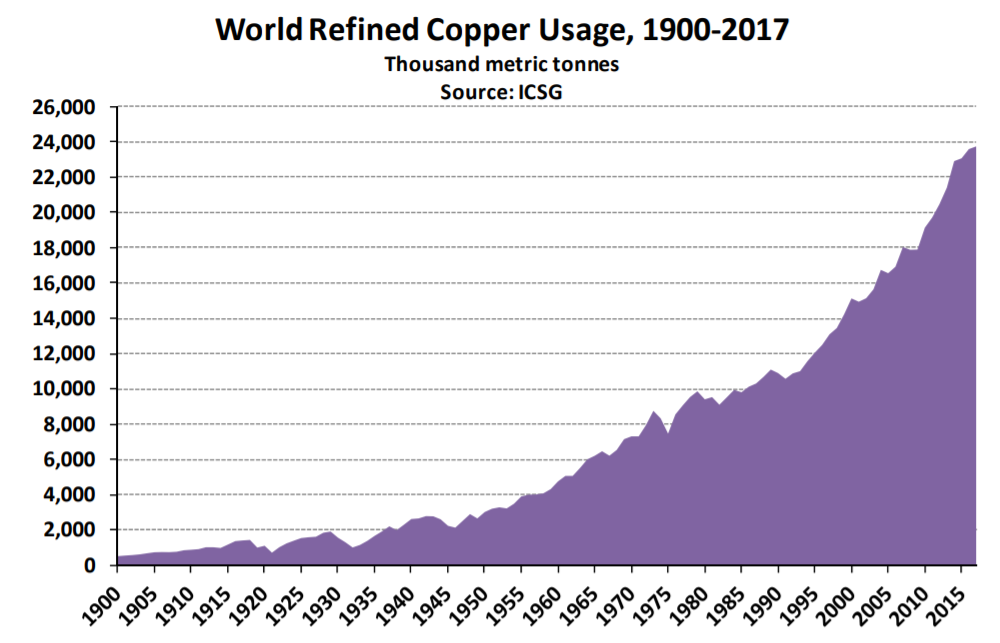
\includegraphics[width=0.8\textwidth]{1/figures/world_refined_copper_usage.png}
%		\caption{Uso del cobre refinado mundial del año 1900 a 2017 (en miles de toneladas). Fuente: \cite{cu_internationalcopper2018}}
%		\label{1:fig}
%	\end{center}
%\end{figure}

%\parencite{cu_internationalcopper2018}.





\section{Formulación del Problema}
Con el objetivo de formular los objetivos de esta investigación, se propusieron las siguientes preguntas.
\subsection{Problema General}
PG:\newcommand{\ProblemaGeneral}{
	¿Cómo el sistema de visión por computadora, que identifica clientes y analiza su comportamiento en una tienda retail, puede recomendar una mejor distribución de productos para optimizar el flujo de clientes y aumentar la eficiencia operativa en tiendas retail en el 2024?
}
\ProblemaGeneral
\subsection{Problemas Espec\'{i}ficos}
\newcommand{\Pbone}{
¿Qué técnicas de visión por computadora se deben usar para identificar y rastrear personas en tiempo real dentro de la tienda?
}
\newcommand{\Pbtwo}{
¿Qué métricas de comportamientos deben analizarse para detectar las zonas más y menos transitadas?
}
\newcommand{\Pbthree}{
¿Cómo debe estructurarse la arquitectura del sistema para procesar video y generar recomendaciones eficientemente?
}
\newcommand{\Pbfour}{
¿Cómo se puede medir el impacto del sistema en la eficiencia operativa y la experiencia del cliente?
}
%\newcommand{\Pbfive}{
%	ES
%}

\begin{itemize}
    \item PE1: {\Pbone}
	\item PE2: {\Pbtwo}
	\item PE3: {\Pbthree}
	\item PE4: {\Pbfour}
	%\item \Pbfive
\end{itemize}

\section{Objetivos de la Investigación}
El objetivo de esta investigación es ofrecer una solución tecnológica que permita a los retails mejorar su eficiencia operativa mediante la implementación de un sistema basado en visión por computadora. Este sistema proporcionará información en tiempo real sobre el comportamiento de los clientes, facilitando decisiones estratégicas para optimizar la disposición de productos, gestionar el inventario y asignar recursos de manera eficiente.
\subsection{Objetivo General}
OG:\newcommand{\ObjetivoGeneral}{
Desarrollar un sistema de visión por computadora que identifique y analice el comportamiento de los clientes dentro de una tienda retail, para recomendar una mejor distribución de productos, con el fin de optimizar el flujo de clientes, aumentar la eficiencia operativa y mejorar la experiencia de compra.
}
\ObjetivoGeneral
\subsection{Objetivos Espec\'{i}ficos}
\newcommand{\Objone}{
Identificar el mejor enfoque para detectar y rastrear personas en tiempo real con alta precisión.
}
\newcommand{\Objtwo}{
Determinar qué indicadores de movimiento y permanencia ayudan a identificar zonas transitadas y menos frecuentadas.
}
\newcommand{\Objthree}{
Definir una arquitectura que procese video y genere recomendaciones de manera rápida y eficiente.
}
\newcommand{\Objfour}{
Establecer métricas para evaluar mejoras en la eficiencia operativa y la satisfacción del cliente.
}
%\newcommand{\Objfive}{
%ghhhg
%}

\begin{itemize}
	\item OE1: {\Objone}
	\item OE2: {\Objtwo}
	\item OE3: {\Objthree}
	\item OE4: {\Objfour}
	%\item {\Objfive}
\end{itemize}

\section{Justificación de la Investigación}

\subsection{Teórica}
La visión por computadora ha emergido como una tecnología clave para automatizar tareas complejas en múltiples sectores, incluyendo el retail. Estudios previos han demostrado que técnicas de inteligencia artificial, como el reconocimiento de imágenes y el análisis de video, permiten identificar patrones de comportamiento en los consumidores y mejorar la disposición de productos en tiendas. Según investigaciones en el ámbito de la distribución minorista, una organización eficiente de los productos, basada en el análisis de datos visuales, puede incrementar las ventas y reducir el tiempo que un cliente invierte en encontrar productos . Además, la teoría de los sistemas recomendadores sugiere que combinar datos históricos de ventas y la interacción del cliente en tiempo real puede mejorar significativamente la satisfacción del cliente y la eficiencia operativa.
La presente investigación se justifica teóricamente porque amplía el conocimiento sobre el uso de la visión por computadora aplicada a entornos de retail familiar, donde la integración de estas tecnologías ha sido limitada por falta de recursos o conocimientos técnicos. Aportará un marco teórico sobre cómo los patrones de movimiento de los clientes, junto con los datos transaccionales, pueden generar recomendaciones dinámicas para la redistribución de productos en un espacio físico limitado.

\subsection{Práctica}
En el contexto de tiendas retail familiares, la implementación de tecnología avanzada, como la visión por computadora, puede transformar procesos actualmente manuales y propensos a errores. Al automatizar el monitoreo y la distribución de productos, las pequeñas tiendas pueden competir más eficazmente con grandes retailers que ya utilizan IA para optimizar sus operaciones. Investigaciones adicionales han demostrado que la optimización de la distribución de productos mediante el análisis del flujo de clientes puede aumentar las ventas hasta en un 15\%. Un estudio realizado por Walmart Labs en 2022 mostró que la aplicación de inteligencia artificial y visión por computadora permitió reducir en un 30\% los problemas de desabastecimiento en sus tiendas, lo que pone de manifiesto el impacto práctico de la tecnología en la optimización operativa. 

La investigación es necesaria para proporcionar una solución práctica y asequible a pequeños negocios que carecen de los recursos de grandes cadenas. Este proyecto de tesis también tiene un enfoque práctico en mejorar la experiencia del cliente al reducir los tiempos de espera y facilitar la disposición de productos más relevante en las zonas de mayor tránsito.

\subsection{Metodológica}. 
La metodología a emplear en esta investigación estará basada en el uso de técnicas de visión por computadora como YOLOv5 o RetinaNet para la detección en tiempo real de clientes dentro de la tienda. El análisis de video se procesará utilizando redes neuronales convolucionales, lo que permite identificar con precisión los patrones de comportamiento y flujo de los clientes. Además, se integrarán datos de ventas y stock en un sistema de recomendación basado en machine learning para sugerir la redistribución de productos. El enfoque metodológico garantiza que los resultados obtenidos sean aplicables no solo en "La Económica", sino también replicables en otros negocios retail de características similares.

La justificación metodológica de este proyecto radica en su innovación al combinar algoritmos de visión por computadora con técnicas de análisis de comportamiento del cliente y optimización de inventario en un solo sistema integrado.
\section{Delimitación del Estudio}
A continuación, se presentará la delimitación espacial, temporal y conceptual.
\subsection{Espacial}
El presente estudio se llevará a cabo en el negocio retail "La Económica", una pequeña tienda minorista ubicada en Lima, Perú. La selección de esta tienda responde a su representatividad dentro del contexto de los pequeños comercios familiares en zonas urbanas de alta densidad. Esta tienda tiene una disposición de productos que sigue un modelo tradicional de retail, pero enfrenta problemas en la gestión y distribución de inventario debido a la falta de recursos tecnológicos. El análisis de la implementación del sistema de visión por computadora se concentrará en este espacio físico, utilizando los datos de comportamiento de los clientes y las características del lugar para optimizar la distribución de productos.

\subsection{Temporal}
El periodo de investigación abarcará desde enero hasta diciembre de 2024. Este periodo permitirá realizar observaciones a lo largo de diferentes estaciones del año, teniendo en cuenta variaciones en el comportamiento del cliente debido a fechas festivas, promociones y cambios estacionales en la demanda de productos. Adicionalmente, se prevé un tiempo de implementación del sistema de visión por computadora, así como un periodo de adaptación para los empleados del negocio.

\subsection{Conceptual}
Para los fines de esta investigación, se definirán los siguientes conceptos clave:
\begin{itemize}
    \item \textbf{Visión por Computadora:} Tecnología que permite a las computadoras y sistemas interpretar y tomar decisiones basadas en imágenes visuales capturadas por cámaras, utilizando algoritmos avanzados de inteligencia artificial para identificar patrones y objetos en tiempo real.
    \item \textbf{Distribución de Productos:} La disposición y organización de los productos dentro de una tienda retail con el fin de optimizar el acceso de los clientes a los productos de mayor demanda y mejorar el flujo de clientes en el establecimiento.
    \item \textbf{Flujo de Clientes:} El patrón de movimiento de los consumidores dentro de la tienda, incluyendo las áreas más frecuentadas, tiempos de permanencia y rutas más comunes que siguen al recorrer el espacio de ventas.
    \item \textbf{Eficiencia Operativa:} La capacidad de un negocio para utilizar sus recursos (tiempo, espacio y personal) de manera óptima, minimizando costos y mejorando la calidad del servicio, lo cual incluye la correcta gestión de inventarios y la disposición eficiente de productos.
\end{itemize}


%\subsection{Matriz de Consistencia}
%A continuación se presenta la matriz de consistencia elaborada para la presente investigación (véase Anexo \ref{1:table}).

